%\section{Backgorund information}

This chaper provides background information that are important in this research.
First two of the most popular overlay networks used in Kubernetes are explaind in detail.
Then the author explain how to utilize multicore CPUs for packet proccessing in Linux.


\section{Container Network}

\subsection{bridge+veth}
\subsection{macvlan, ipvlan}
\subsection{hostnetwork}


\section{Overlay Network}


\subsubsection{Overlay Network}\label{sec:overlay_network}

In order to discuss load balancer for container cluster, the knowledge of the overlay network is essential.
We briefly explain an abstract concept of overlay network in this subsection.

\begin{figure}[tb]
\centering
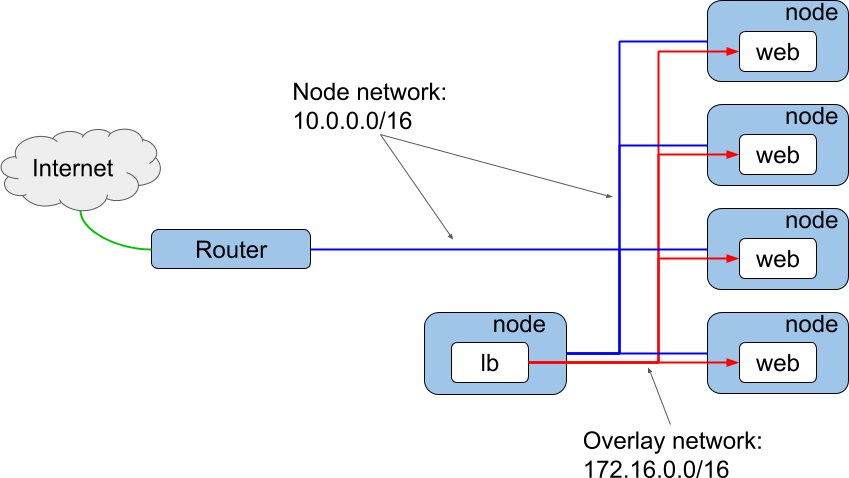
\includegraphics[width=0.8\columnwidth]{Figs/overlay.png}
\caption{The network architecture of an exemplified container cluster system. }

  A load balancer(lb) pod(the white box with "lb") and web pods are running on nodes(the blue boxes).
  The traffic from the internet are forwarded to the lb pod by the upstream router using the node network,
  and the distributed to web pods using the overlay network.

\label{fig:overlay}
\end{figure}

Fig.~\ref{fig:overlay} shows schematic diagram of network architecture of a container cluster system. 
Suppose we have a physical network(node network) with IP address range of 10.0.0.0/16 and an overlay network with IP address range of 172.16.0.0/16.
The node network is the network for nodes to communicate with each other.
The overlay network is the network setups for containers to communicate with each other.
An overlay network typically consists of appropriate routing tables on nodes, and optionally of tunneling setup using ipip or vxlan.
The upstream router usually belongs to the node network.
When a container in the Fig.~\ref{fig:overlay} communicates with any of the nodes, it can use its IP address in 172.16.0.0/16 IP range as a source IP, since every node has proper routing table for the overlay network.
When a container communicates with the upstream router that does not have routing information regarding the overlay network, the source IP address must be translated by Source Network Address Translation(SNAT) rules on the node the container resides.

The SNAT caused a problem when we tried to co-host multiple load balancer containers for different services on a single node, and let them connect the upstream router directly.
This was due to the fact that the BGP agent used in our experiment only used the source IP address of the connection to distinguish the BGP peer.
The agent behaved as though different BGP connections from different containers belonged to a single BGP session because the source IP addresses were identical due to the SNAT.

There many overlay network implementations.
The author investigated two of the popular ones to see how it works.


\subsection{General concept}

\subsection{Flannel}

We used flannel to build the Kubernetes cluster used in our experiment.
Flannel has three types of backend, {\it i.e.}, operating modes, named host-gw, vxlan, and udp\cite{CoreOSFlannelBackend}.

In the host-gw mode, the flanneld installed on a node simply configures the routing table 
based on the IP address assignment information of the overlay network, which is stored in the etcd. 
When a {\em pod} on a node sends out an IP packet to {\em pods} on the different node, 
the former node consults the routing table and learn that the IP packet should be sent out to the latter.
Then, the former node forms Ethernet frames containing the destination MAC address of the latter node 
without changing the IP header, and send them out.

In the case of the vxlan mode, flanneld creates the Linux kernel's vxlan device, flannel.1. 
Flanneld will also configures the routing table appropriately based on the information stored in the etcd.
When {\em pods} on different nodes need to communicate, the packet is routed to flannel.1.
The vxlan functionality of the Linux kernel identify the MAC address of flannel.1 device on the destination node,
then form an Ethernet frame toward the MAC address.
The vxlan then encapsulates the Ethernet frame in a UDP/IP packet with a vxlan header, after which the IP packet is eventually sent out.

In the case of udp mode, flanneld creates the tun device, flannel0, and configures the routing table.
The flannel0 device is connected to the flanneld daemon itself.
An IP packet routed to flannel0 is encapsulated by flanneld, and eventually sent out 
to the appropriate node. 
The encapsulation is done for IP packets.

Figure~\ref{fig:flannel-packet-diagram} shows the schematic diagrams of frame formats for three backends modes of the flannel overlay network. 
The MTU sizes in the backends, assuming the MTU size without encapsulation is 1500 bytes, are also presented.
Since packets are not encapsulated in the host-gw mode, the MTU size remains 1500 bytes.
An additional 50 bytes of header is used in the vxlan mode, thereby resulting in an MTU size of 1450 bytes.
In the case of the udp mode, only 28 bytes of header are used for encapsulation, which results in an MTU size of 1472 bytes.

\begin{figure}
  \centering
  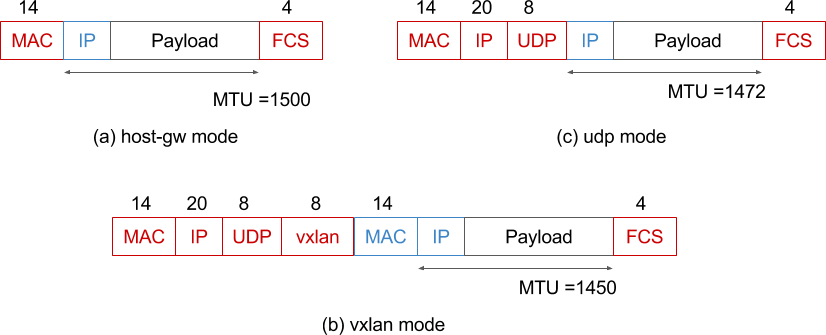
\includegraphics[width=0.8\columnwidth]{Figs/flannel-packet-diagram}
  \caption{Frame diagram}
  \label{fig:flannel-packet-diagram}
\end{figure}

Performance of the load balancers can be influenced by the overhead of encapsulation. 
Thus, the host-gw mode, where there is no overhead due to encapsulation, 
results in the best performance levels as is shown in Chapter~\ref{chapter:portablelb}.
However, the host-gw mode has a significant drawback that prohibit it to work correctly in cloud platforms. 
Since the host-gw mode simply sends out a packet without encapsulation, if there is a cloud gateway between nodes, 
the gateway cannot identify the proper destination, thus drop the packet.

\begin{table}
  \centering
  \begin{tabular}{lccc}
    \toprule
    mode & On-premise & GCP & AWS \\
    \midrule
    host-gw & OK & NG & NG \\
    vxlan & OK & OK & OK \\
    udp & OK & OK & OK \\
    \bottomrule
\end{tabular}

  \caption{Viable flannel backend modes. In cloud environment tunnelig using vxlan or udp is needed.}
  \label{tab:Viable flannel backends}
\end{table}

We conducted an investigation to determine which of the flannel backend mode would be usable on AWS, GCP, and on-premise data centers.
The results are summarized in Table~\ref{tab:Viable flannel backends}. 
In the case of GCP, an IP address of {\tt /32} is assigned to every VM host and 
every communication between VMs goes through GCP's gateway.
As for AWS, the VMs within the same subnet communicate directly, while the VMs in different subnets communicate via the AWS's gateway.
Since the  gateways do not have knowledge of the flannel overlay network, they drop the packets; thereby, 
they prohibit the use of the flannel host-gw mode in those cloud providers.  

In our experiment, we compared the performance of load balancers when different flannel backend modes were used. 

%% \paragraph{\bf host-gw}
%% \paragraph{\bf vxlan}
%% \paragraph{\bf udp}

\subsection{Calico}
[Filled in later]
%% \paragraph{\bf no-tunnel}
%% \paragraph{\bf ipip}


\section{Multicore Packet Proccessing}

Recently, the performance of CPUs are improved significantly due to the development of multi-core CPUs.
One of the top of the line server processors from Intel now includes up to 28 cores in a single CPU.
In order to enjoy the benefits of multi-core CPUs in communication performance, 
it is necessary to distribute the handling of interrupts from the NIC and the IP protocol processing to the available physical cores.

\mytodo[inline]{Write about rps,rfs,xfs}

\subsection{rss}

Receive Side Scaling (RSS)\cite{TomHerbert} is a technology 
to distribute handling of the interrupt from NIC queues to multiple CPU cores.
Subsequently, Receive Packet Steering (RPS)\cite{TomHerbert} distributes the IP protocol processing 
to multiple CPU cores by issuing inter core software interrupts.

Since load balancer performance levels could be affected by these technologies,
we conducted an experiment to determine how load balancer performance level change depending on the RSS and RPS settings.
The following shows how RSS and RPS are enabled and disabled in our experiment. 
The NIC used in our experiment is Broadcom BCM5720, which has four rx-queues and one tx-queue.
Figure~\ref{fig:rx-queue} shows the interrupt request (IRQ) number assignments to those NIC queues.

\begin{figure}
\centering
\begin{minipage}{0.5\columnwidth}
\begin{verbatim}
81: eth0-tx-0
82: eth0-rx-1
83: eth0-rx-2
84: eth0-rx-3
85: eth0-rx-4
# obtained from /proc/interrupts 
\end{verbatim}
\end{minipage}
\caption{RX/TX queues of the hardware}
\label{fig:rx-queue}
\end{figure}

When packets arrive, they are distributed to these rx-queues depending on the flow each packet belongs to.
Each receive queue has a separate IRQ associated with it. The NIC triggers
this to notify a CPU when new packets arrive on the given queue.
Then, the notified CPU handles the interrupt, and performs the protocol processing. 
According to the \cite{TomHerbert}, the CPU cores allowed to be notified is controlled by setting 
a hexadecimal value corresponding to the bit maps indicating the allowed CPU cores in \enquote{/proc/irq/\$irq\_number /smp\_affinity}.
%
For example, in order to route the interrupt for eth0-rx-1 to CPU0, 
we should set \enquote{/proc/irq/82/smp\_affinity} 
to binary number {\tt 0001}, which is 1 in hexadecimal value.
Further, in order to route the interrupt for eth0-rx-2 to CPU1, we 
should set \enquote{/proc/irq/83/smp\_affinity} 
to binary number {\tt 0010}, which is 2 in hexadecimal value.

We refer the setting to distribute interrupts from four rx-queues to CPU0, CPU1, CPU2 and CPU3 as {\tt RSS = on}. 
It is configured as the following setting: 

\begin{center}
\begin{minipage}{0.6\columnwidth}
\begin{Verbatim}[commandchars=\\\{\}]

\underline{\textbf{RSS=on}}
echo 1 > /proc/irq/82/smp_affinity
echo 2 > /proc/irq/83/smp_affinity
echo 4 > /proc/irq/84/smp_affinity
echo 8 > /proc/irq/85/smp_affinity

\end{Verbatim}
\end{minipage}
\end{center}

On the other hand, {\tt RSS = off} means that an interrupt from any rx-queue is routed to CPU0. 
It is configured as the following setting:

\begin{center}
\begin{minipage}{0.6\columnwidth}
\begin{Verbatim}[commandchars=\\\{\}]

\underline{\textbf{RSS=off}}
echo 1 > /proc/irq/82/smp_affinity
echo 1 > /proc/irq/83/smp_affinity
echo 1 > /proc/irq/84/smp_affinity
echo 1 > /proc/irq/85/smp_affinity

\end{Verbatim}
\end{minipage}
\end{center}

%In this case, interrupt from any of rx-queue is routed to CPU0.
\subsubsection{rps}

The RPS distributes IP protocol processing by placing the packet
on the desired CPU's backlog queue and wakes up the CPU using inter-processor interrupts.
We have used the following settings to enable the RPS:

\begin{center}
\begin{minipage}{0.8\columnwidth}
\begin{Verbatim}[commandchars=\\\{\}]

\underline{\textbf{RPS=on}}
echo fefe > /sys/class/net/eth0/queues/rx-0/RPS_cpus
echo fefe > /sys/class/net/eth0/queues/rx-1/RPS_cpus
echo fefe > /sys/class/net/eth0/queues/rx-2/RPS_cpus
echo fefe > /sys/class/net/eth0/queues/rx-3/RPS_cpus

\end{Verbatim}
\end{minipage}
\end{center}

Since the hexadecimal value \enquote{fefe} represented as \enquote{1111 1110 1111 1110} in binary, 
this setting will allow distributing protocol processing to all of the CPUs, except for CPU0 and CPU8.
In this paper, we will refer this setting as {\tt RPS = on}.
%
On the other hand, {\tt RPS = off} means that no CPU is allowed for RPS. 
Here, the IP protocol processing is performed on the CPUs the initial hardware interrupt is received.
It is configured as the following settings:

\begin{center}
\begin{minipage}{0.8\columnwidth}
\begin{Verbatim}[commandchars=\\\{\}]

\underline{\textbf{RPS=off}}
echo 0 > /sys/class/net/eth0/queues/rx-0/RPS_cpus
echo 0 > /sys/class/net/eth0/queues/rx-1/RPS_cpus
echo 0 > /sys/class/net/eth0/queues/rx-2/RPS_cpus
echo 0 > /sys/class/net/eth0/queues/rx-3/RPS_cpus

\end{Verbatim}
\end{minipage}
\end{center}

The RPS is especially effective when the NIC does not have multiple receive queues or when the number of queues is 
much smaller than the number of CPU cores. 
That was the case of our experiment, where we had a NIC with only four rx-queues, 
while there was a CPU with eight physical cores.

\section{Linux vritual server}

In order to demonstrate a software load balancer that is runnable in any environment, the ipvs is containerized.  
In addition to that the proposed load balancer uses two other components, keepalived, and a controller. 
These components are placed in a single Docker container image.
The ipvs is a Layer-4 load balancer capability, which is included in the Linux kernel 2.6.0 released in 2003 or later, 
to distribute incoming Transmission Control Protocol(TCP) traffic to 
{\em real servers}\footnote{The term, {\em real servers} refers to worker servers that will respond to incoming traffic, 
in the original literature\cite{Zhang2000}. We will also use this term in the similar way.}\cite{Zhang2000}. 
For example, ipvs distributes incoming Hypertext Transfer Protocol(HTTP) traffic destined for a single destination IP address, 
to multiple HTTP servers(e.g. Apache HTTP or nginx) running on multiple nodes in order to improve the performance of web services.
Keepalived is a management program that performs health checking for {\em real servers}
and manages ipvs balancing rules in the kernel accordingly.
It is often used together with ipvs to facilitate ease of use.
The controller is a daemon that periodically monitors the {\em pod} information on the master, 
and it performs various actions when such information changes.
Kubernetes provides ingress controller framework as the Go Language(Golang) package to implement the controllers. 
We implement a controller program that feeds {\em pod} state changes to keepalived 
using this framework. 

\mytodo[inline]{Write about ipvs}


\section{Summary}
\mytodo[inline]{Write summary for background}
